\noindent\textbf{Precipitation perturbation.}
\vspace{0.5cm}

Figure~\ref{fig:ppt_cdf_04} shows the effect of the Gaussian multiplier scheme on the precipitation input. The left panel displays the empirical \ac{cdf} of hourly precipitation values: the 5--95\,\% percentile envelope of the 2000 perturbed series closely brackets the original record, with the narrowing band at higher precipitation values reflecting the multiplicative nature of the perturbation. The right panel shows the accumulated precipitation over the simulation period; all 2000 perturbed traces remain visually indistinguishable from the original at this scale, confirming that the random multipliers cancel out over long aggregation periods. The mean absolute relative change (MARC) across series averages $6.62\,\%$ (range: $6.14$--$7.04\,\%$), consistent with a one-sigma noise level of roughly $5\,\%$ at each time step.

\begin{figure}[!ht]
    \centering
    \begin{minipage}{0.49\textwidth}
        \centering
        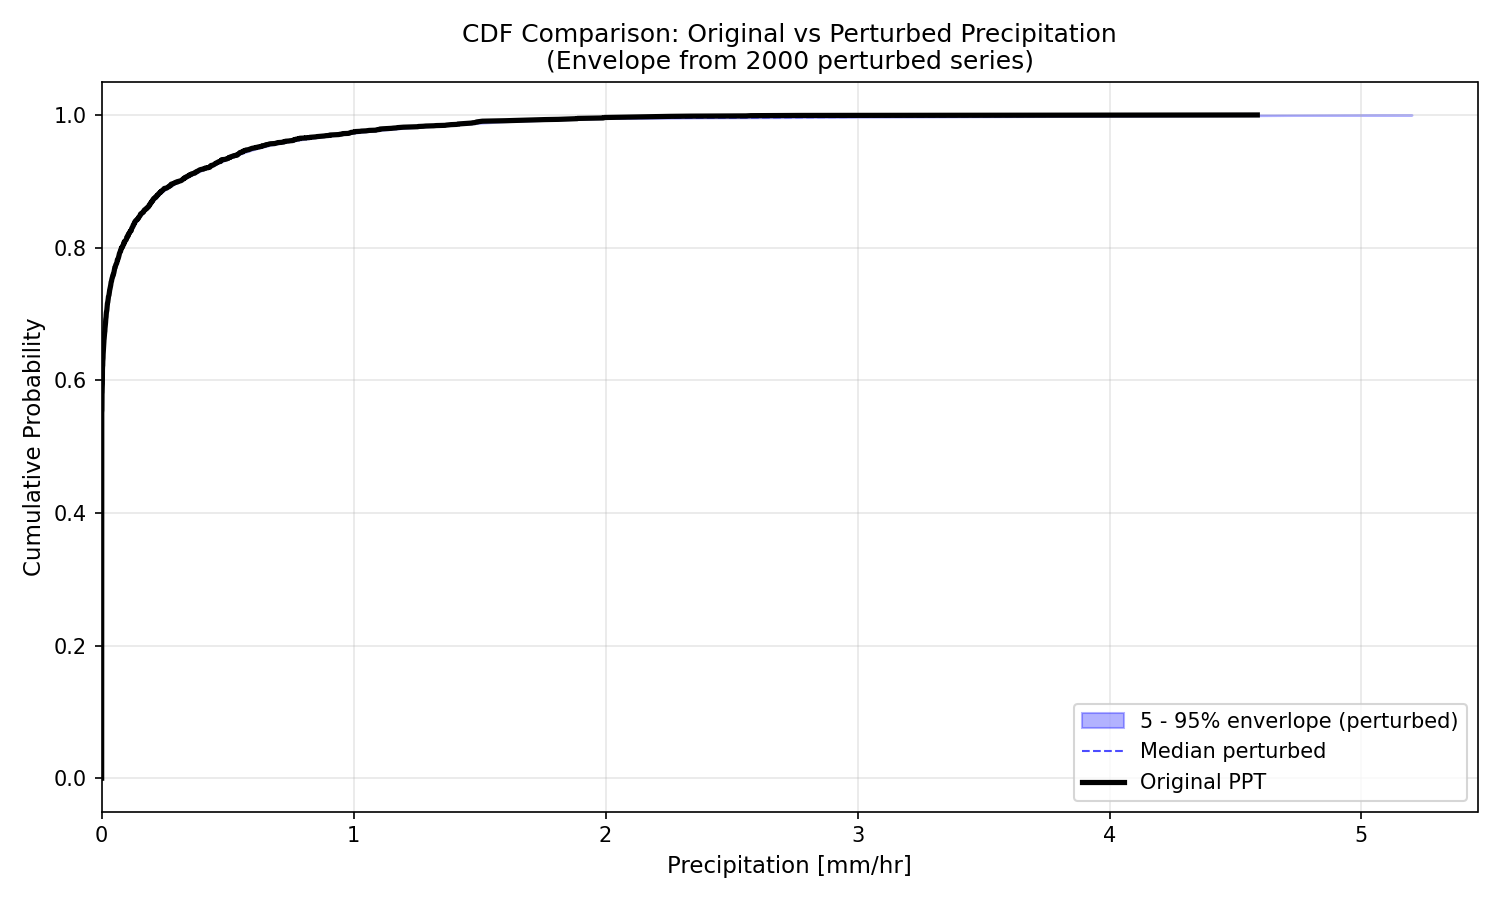
\includegraphics[width=\textwidth]{Figures/Ass_04/ppt_cdf_comparison.png}
    \end{minipage}
    \hfill
    \begin{minipage}{0.49\textwidth}
        \centering
        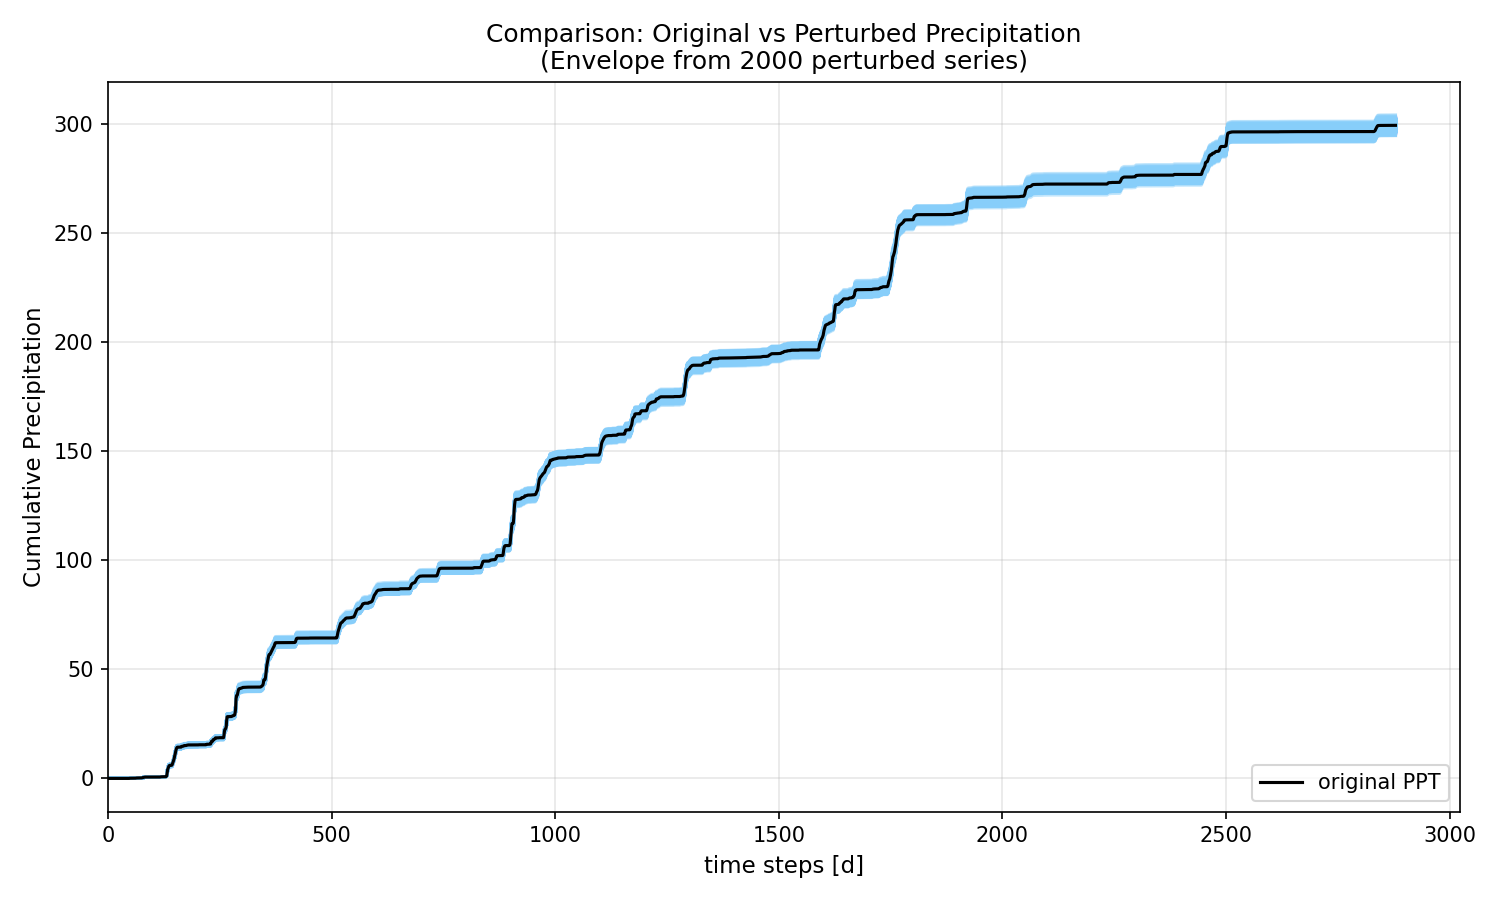
\includegraphics[width=\textwidth]{Figures/Ass_04/ppt_cdf_comparison_two.png}
    \end{minipage}
    \caption{Precipitation perturbation. Left: empirical CDF of hourly precipitation values showing the 5--95\,\% envelope of 2000 perturbed series against the original record. Right: cumulative precipitation over the simulation period for all perturbed series (light blue) and the original (black).}
    \label{fig:ppt_cdf_04}
\end{figure}

\noindent\textbf{OFV distributions.}
\vspace{0.5cm}

Figure~\ref{fig:ofv_cdf_04} shows the CDF of the \ac{ofv} across the 2000 series for both experiments. When the fixed reference parameter set is applied, the mean \ac{ofv} increases only marginally from the reference value of $0.0923$ to $0.0927$ (mean \ac{nse}: $0.9073$). With recalibration, the mean \ac{ofv} is reduced slightly further to $0.0925$ (mean \ac{nse}: $0.9075$). The two CDF curves are nearly congruent, indicating that the overall spread of \ac{ofv} values is not substantially reduced by recalibration: the 90\,\% range (5th to 95th percentile) is $0.0060$ for the reference-parameter run and $0.0062$ for the recalibrated run.

The fraction of perturbed series that outperformed the reference \ac{ofv} by chance is $834/2000$ ($41.7\,\%$) when reference parameters are used, rising modestly to $933/2000$ ($46.6\,\%$) after recalibration. The finding that a large fraction of random perturbations improve performance without any recalibration suggests that the original calibration period does not represent the global optimum for the true precipitation field, and that modest input noise occasionally shifts the model closer to a better-performing state.\\

\begin{figure}[!ht]
    \centering
    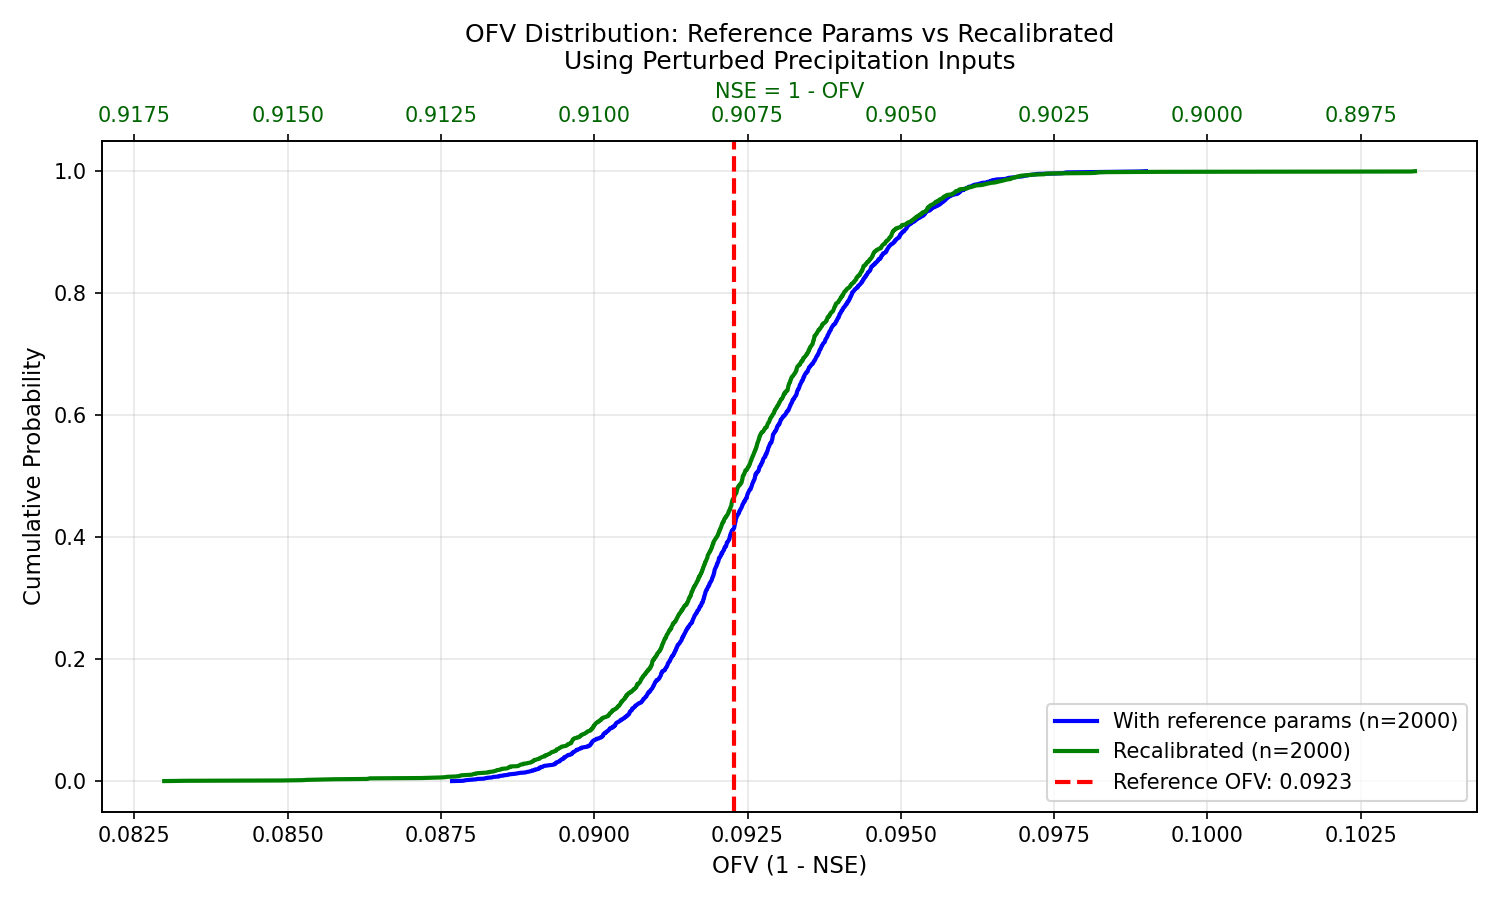
\includegraphics[width=0.85\textwidth]{Figures/Ass_04/ofv_cdfs.png}
    \caption{\Ac{ofv} CDFs for all 2000 perturbed series run with the reference parameter set (blue) and after recalibration (green). The red dashed line marks the reference \ac{ofv} of $0.0923$. The top axis shows the equivalent \ac{nse}.}
    \label{fig:ofv_cdf_04}
\end{figure}

\noindent\textbf{MARC versus OFV scatter.}
\vspace{0.5cm}

Figure~\ref{fig:scatter_marc_04} shows the scatter of \ac{ofv} against the per-series MARC for both the reference-parameter (left) and recalibrated (right) runs. In both panels the correlation between MARC and \ac{ofv} is negligible ($r \approx 0.0$), which is expected: because all multipliers are drawn from the same distribution with the same variance, the MARC is nearly constant across series (coefficient of variation below $2.5\,\%$) and carries almost no predictive information about model performance. The \ac{ofv} spread observed in both panels is therefore attributable to the particular realisation of the random perturbation rather than to its average magnitude.\\

\begin{figure}[!ht]
    \centering
    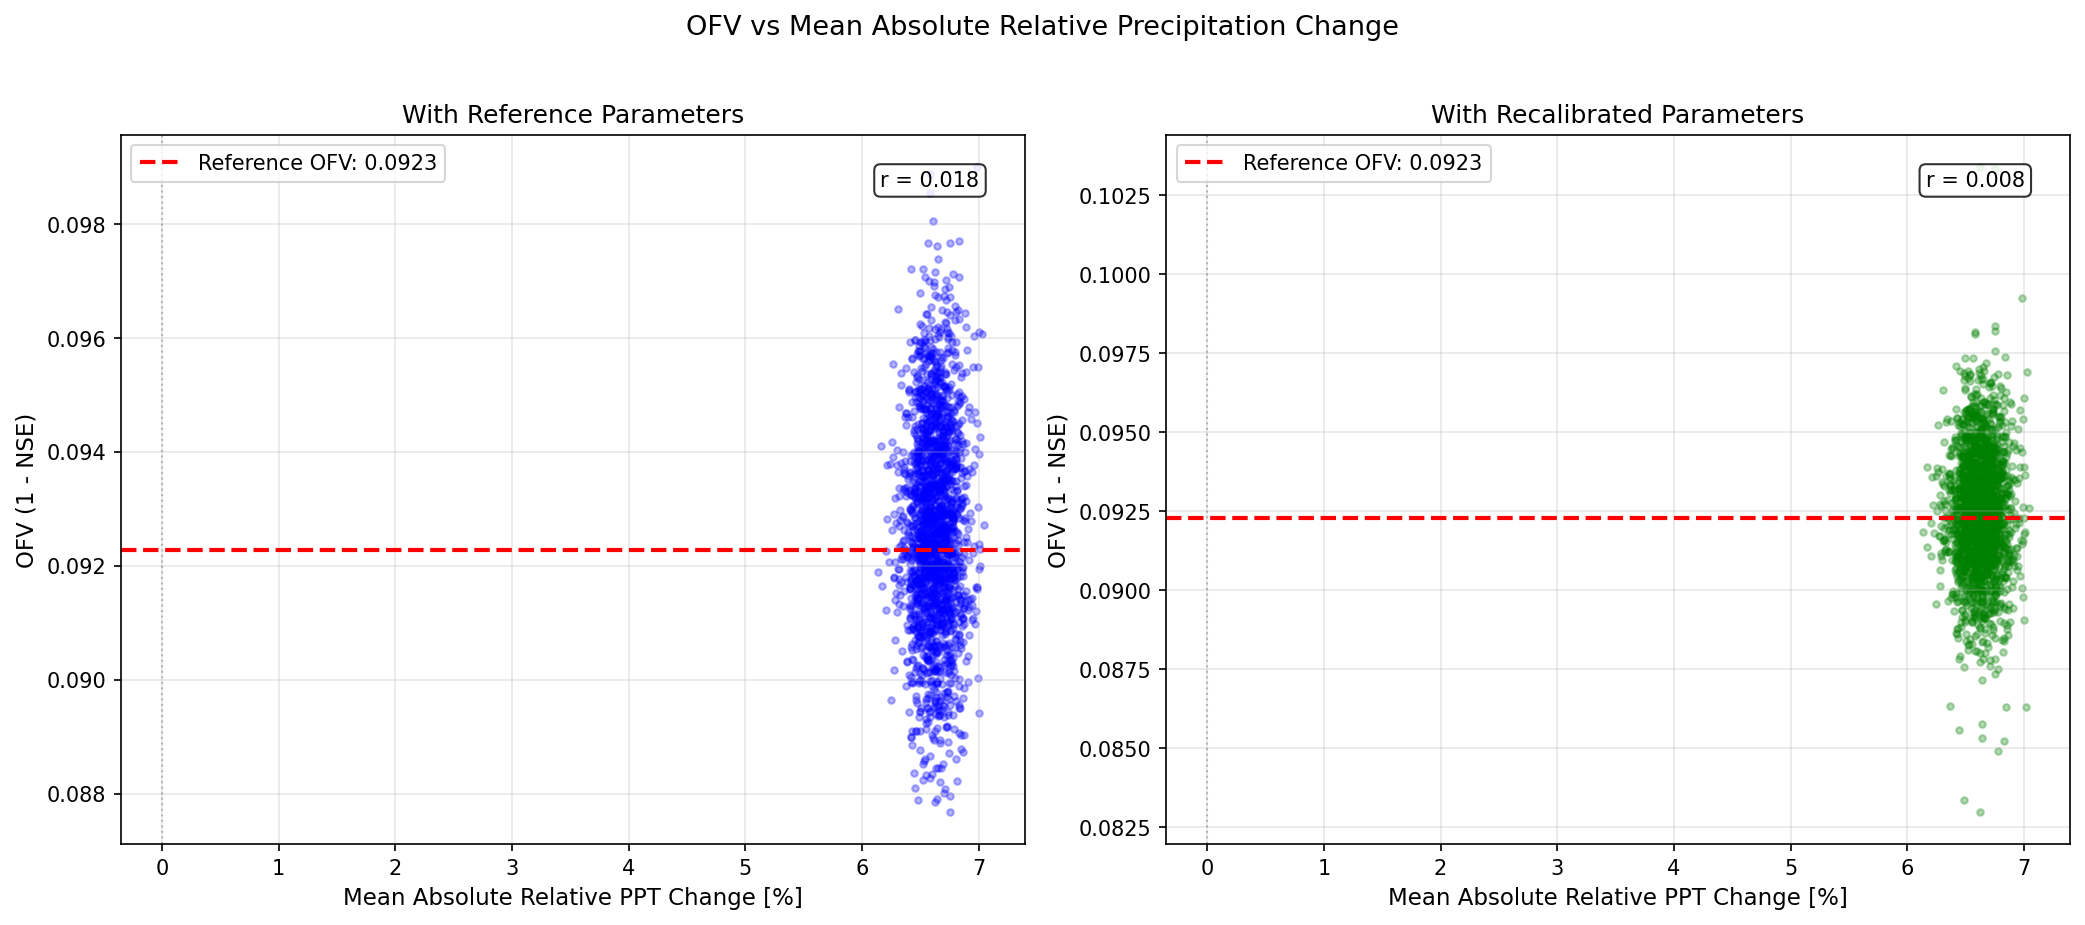
\includegraphics[width=\textwidth]{Figures/Ass_04/scatter_ppt_change_vs_ofv.png}
    \caption{Scatter plot of mean absolute relative precipitation change (MARC, $x$-axis) versus \ac{ofv} for the reference-parameter run (left, blue) and the recalibrated run (right, green). The red dashed line marks the reference \ac{ofv}. Near-zero correlation in both panels confirms that MARC is not a meaningful predictor of performance degradation in this experiment.}
    \label{fig:scatter_marc_04}
\end{figure}

\noindent\textbf{Recalibration versus reference parameters.}
\vspace{0.5cm}

Figure~\ref{fig:scatter_ofv_04} plots OFV$_\text{recal}$ against OFV$_\text{ref}$ for all 2000 series. Most points lie below the 1:1 line, confirming that recalibration improves the \ac{ofv} for $1908/2000$ series ($95.4\,\%$). The improvement is small in absolute terms (mean reduction of $0.0002$) and the points remain tightly clustered around the 1:1 line, indicating that the reference parameter set is already close to optimal for each perturbed input, with the \ac{de} optimizer finding only marginal gains. Because the mean performance loss induced by the perturbation itself is negligible ($\Delta\text{OFV} = +0.0004$), the recalibration improvement cannot be interpreted as compensation for input-induced degradation; rather, it more likely reflects series-specific overfitting by the optimizer and minor differences between the reference \ac{de} run and the warm-started recalibration.

\begin{figure}[!ht]
    \centering
    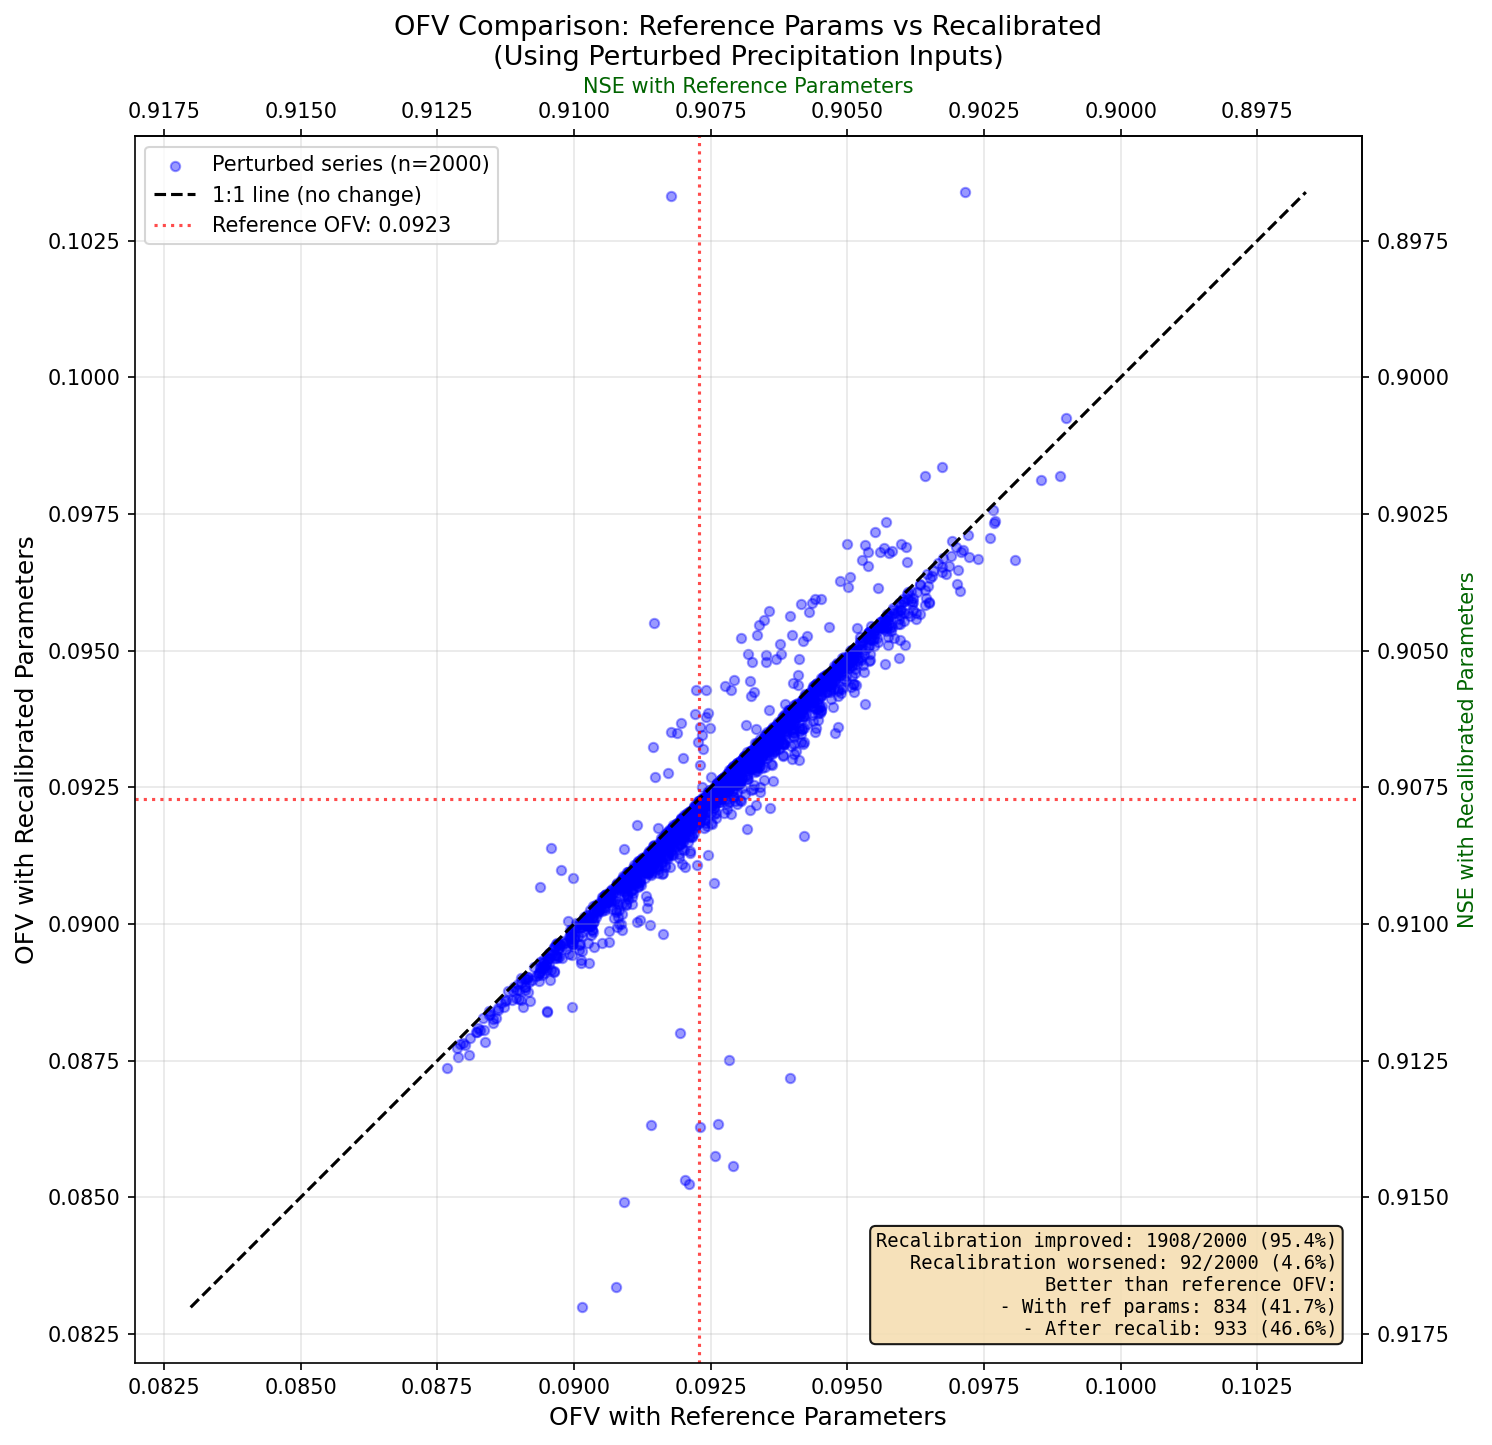
\includegraphics[width=0.75\textwidth]{Figures/Ass_04/scatter_ofv_ref_vs_recalibrated.png}
    \caption{Scatter plot of \ac{ofv} with reference parameters ($x$-axis) versus \ac{ofv} after recalibration ($y$-axis) for all 2000 perturbed series. The black dashed line is the 1:1 reference. Points below the line indicate improvement through recalibration ($95.4\,\%$ of series). The secondary axes show the equivalent \ac{nse} values.}
    \label{fig:scatter_ofv_04}
\end{figure}

\noindent\textbf{Parameter uncertainty under input perturbation.}
\vspace{0.5cm}

Figure~\ref{fig:param_cdf_04} shows the empirical CDFs of all 17 free parameters across the 2000 recalibrations, with the reference value from Assignment~1 indicated by a vertical dashed line. The degree of spread varies substantially between parameters. The most sensitive to input uncertainty are \texttt{lrr\_dre}, \texttt{urr\_ndr} (excluding \ac{mp} with no change), reflecting parameters that are tightly distributed around their reference values. Small changes in those parameters alter reservoir and subsurface storage dynamics during calibration. Suggesting these are robustly identifiable even under perturbed inputs. By contrast, upper-reservoir parameter, such as \texttt{urr\_tdr} and \texttt{urr\_tdh} varie over the total parameter range and their signal is easily obscured by precipitation noise.\\


\begin{figure}[!ht]
    \centering
    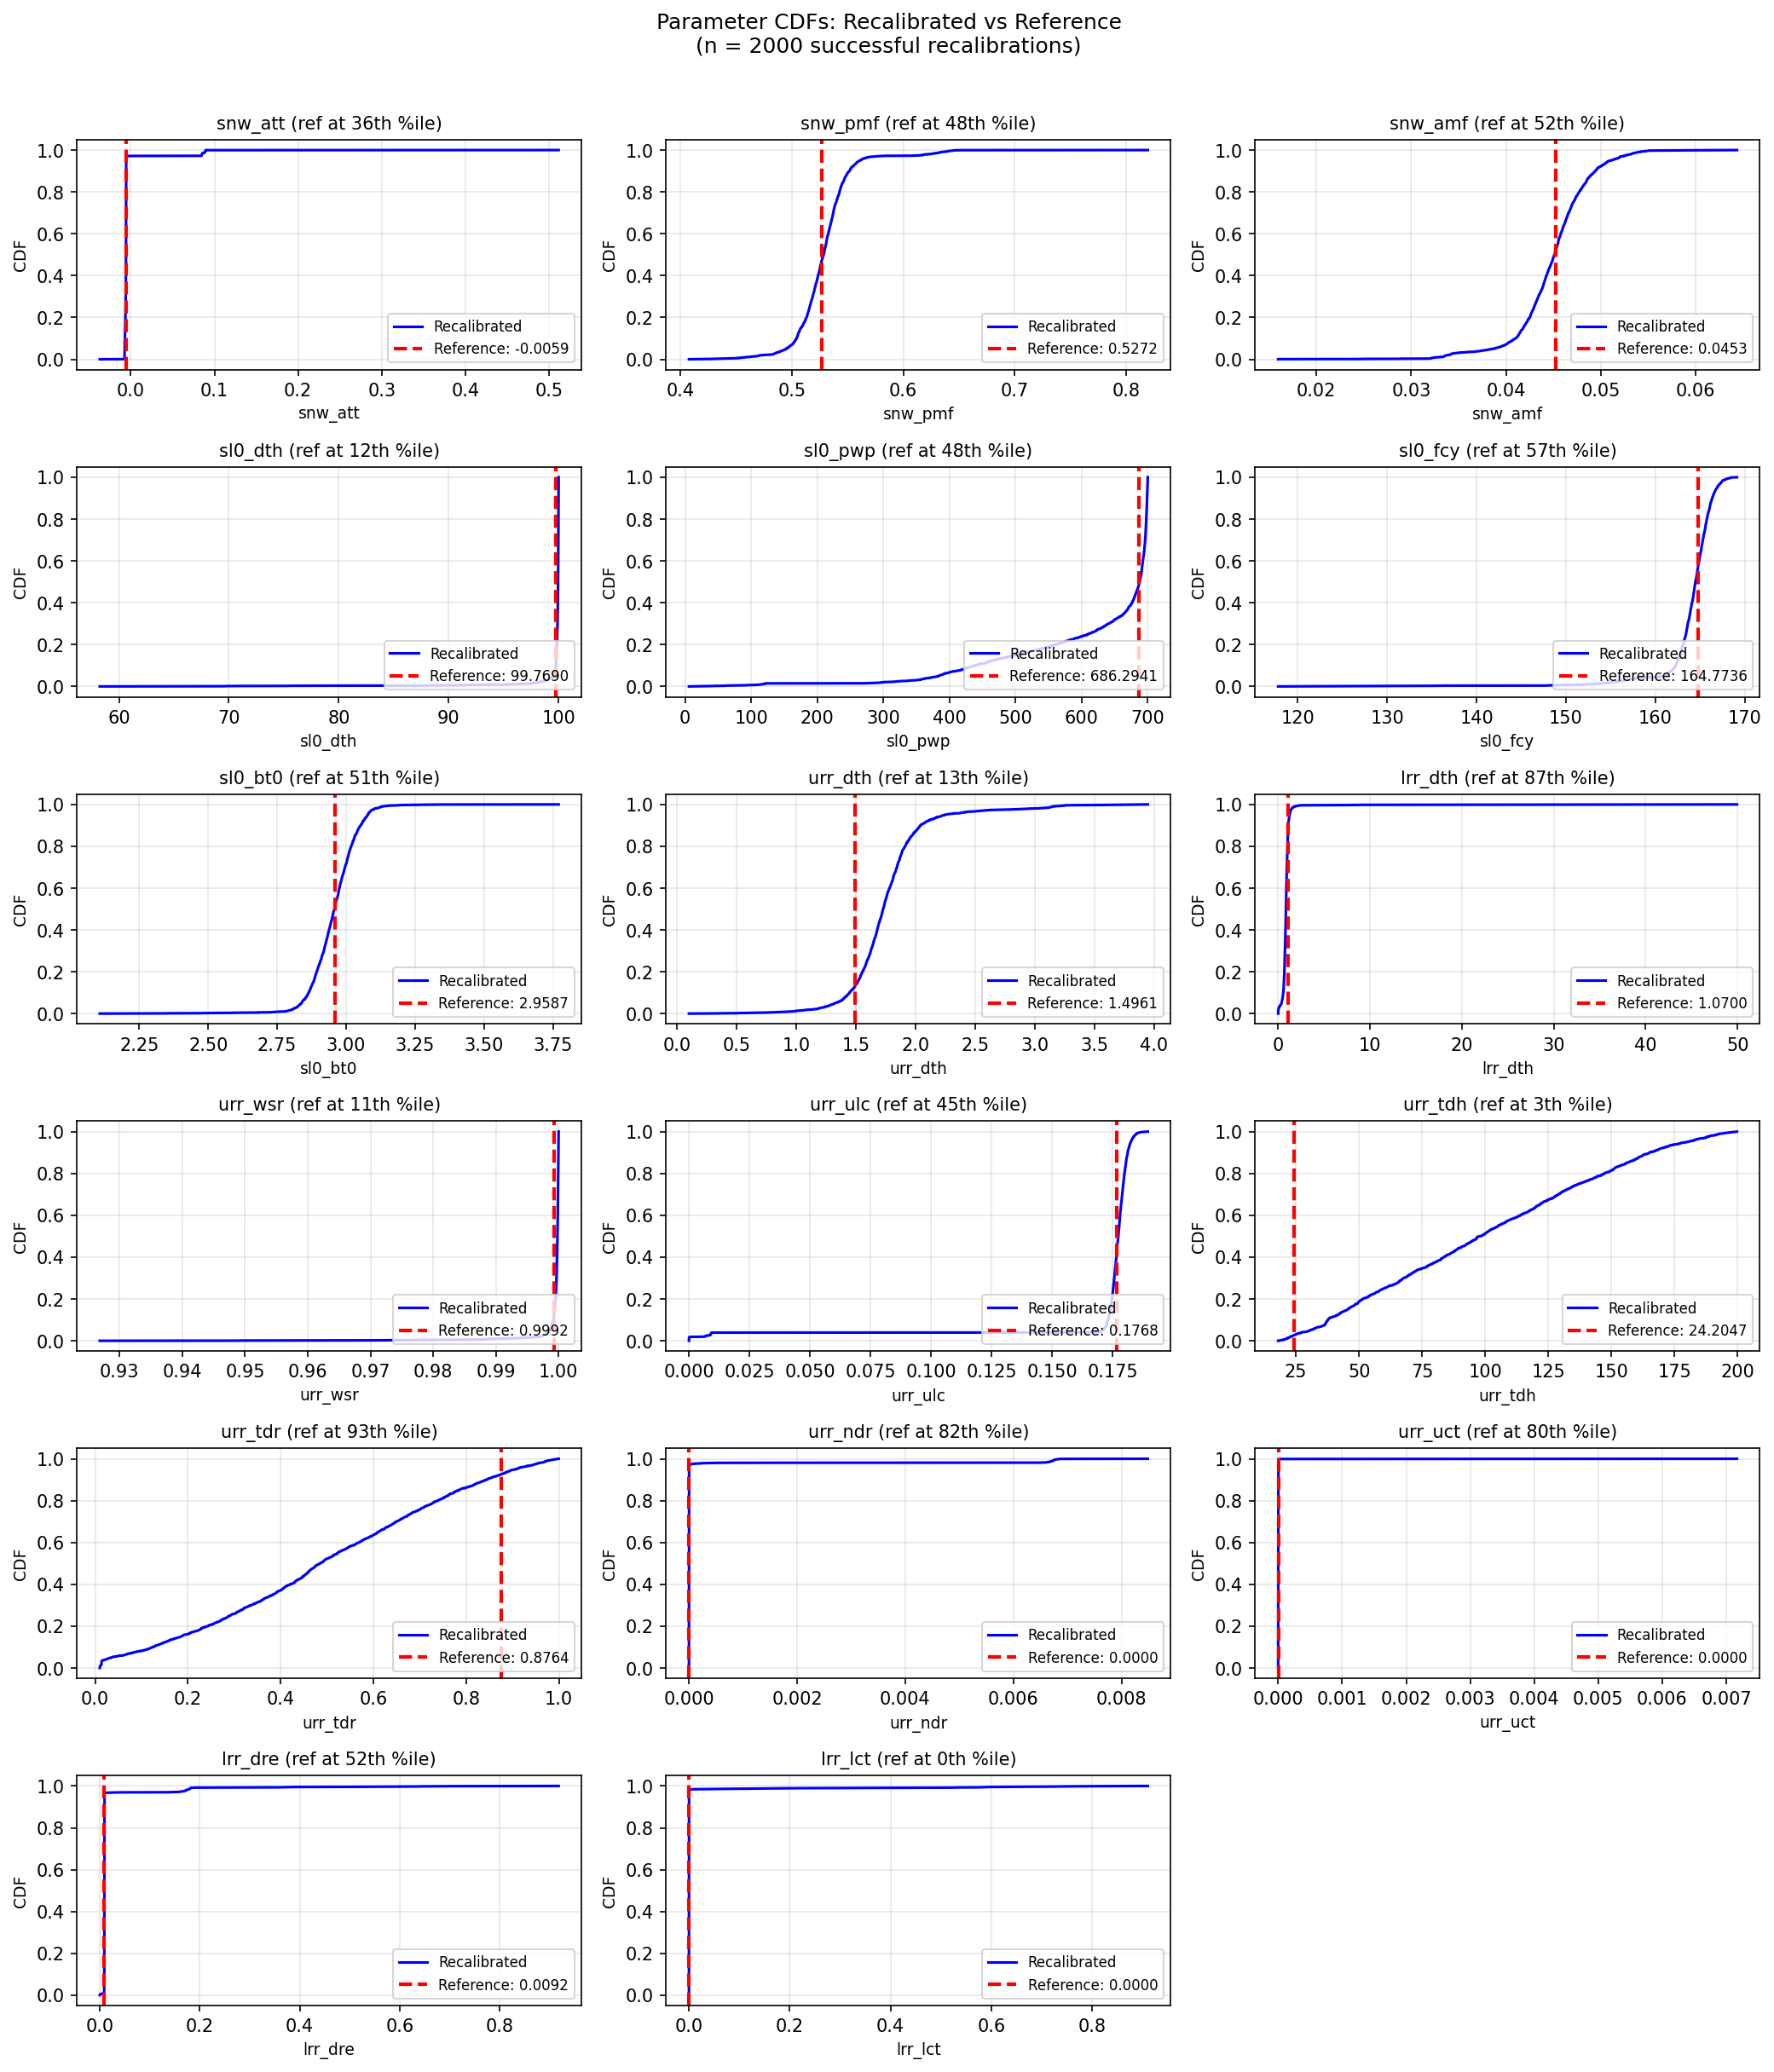
\includegraphics[width=\textwidth]{Figures/Ass_04/parameter_cdfs.png}
    \caption{Empirical CDFs of the 17 free parameters across 2000 recalibrated runs. The red dashed vertical line marks the reference value from Assignment~1. Panels are ordered by module: snow (top), soil layer, upper reservoir, and lower reservoir (bottom).}
    \label{fig:param_cdf_04}
\end{figure}

\noindent\textbf{Comparison with Oudin et al.~(2006).}
\vspace{0.5cm}

The results are broadly consistent with \textcite{Oudin.2006}. They found that randomly corrupted inputs degrade model efficiency only modestly on average, because the optimizer can absorb part of the noise through parameter adjustment, while the remaining degradation reflects irreducible input-induced output variance. The same pattern is observed here: mean performance loss with fixed parameters is negligible ($\Delta\text{NSE} = -0.0004$) and recalibration reduces the mean \ac{ofv} by a further $0.0002$ at the cost of substantially increased parameter uncertainty for \texttt{urr\_tdh} and \texttt{lrr\_dth}. The present analysis uses only random (zero-mean) perturbations; \textcite{Oudin.2006} additionally tested systematically biased inputs and found that bias introduces a persistent performance loss that recalibration cannot fully compensate, which is not testable with the current experimental design. Taken together, the results highlight that input uncertainty during calibration provides more robust parameter estimates and better-characterized prediction uncertainty bounds, particularly for the slow-response reservoir parameters that are most affected by precipitation errors.
\\
Literature findings also indicate that when input rainfall data contains errors, the model attempts to limit the impact of erroneous rainfall on runoff calculations by increasing the capacity of the SMA basin, which can be applied in our assignment report:if we observe a shift in the CDF of parameters after recalibration, then we can use this theory to explain it: the model is "masking" the uncertainty in the input data by adjusting its internal functions, such as storage or exchange.In \textcite{Oudin.2006}, it is referred to as the \textbf{Parameter Compensation Mechanism}, which comes from absorption theory.


\\

%% one more comparison about optimization method
Finally,\cite{Oudin.2006} differs from our assignment in one further respect concerning the optimisation algorithm.
\subsubsection*{Comparison of Optimization Algorithms}

\begin{itemize}
    \item \textbf{Optimization Algorithm Type:} 
    Oudin (2006) employed \textbf{Gradient Search}, which is a local optimization technique. In contrast, our HBV model uses \textbf{Differential Evolution}, a heuristic global optimization approach.
    
    \item \textbf{Search Features:}
    The Gradient Search is limited to \textbf{local optimization}, making it highly efficient but narrow in scope. Differential Evolution provides \textbf{global optimization} capabilities, offering a more comprehensive search of the parameter space.
    
    \item \textbf{Advantages (Pros):}
    \begin{itemize}
        \item \textit{Gradient Search:} Characterized by fast convergence speeds.
        \item \textit{Differential Evolution:} Capable of escaping local optima, significantly more robust, and more likely to identify the true global optimum.
    \end{itemize}
    
    \item \textbf{Disadvantages (Cons):}
    \begin{itemize}
        \item \textit{Gradient Search:} Extremely prone to getting trapped in local optima, which can lead to biased parameter estimation.
        \item \textit{Differential Evolution:} While robust, it is often more computationally intensive (no other significant findings temporally).
    \end{itemize}
\end{itemize}